\documentclass[a4paper]{article}
\usepackage[utf8]{inputenc}
\usepackage[T1]{fontenc}

\usepackage{lmodern}
\usepackage[]{fullpage}

\usepackage{graphicx}
\graphicspath{ {../Plots/} }

\begin{document}
\title{\vspace{-2.5cm}Scalability Of Clustering Algorithm}
\author{Silas Nyboe Ørting}
\maketitle
\thispagestyle{empty}

\input{README.tex}

\pagebreak
\section{Plots}
\begin{figure}[!h]
  \centering
  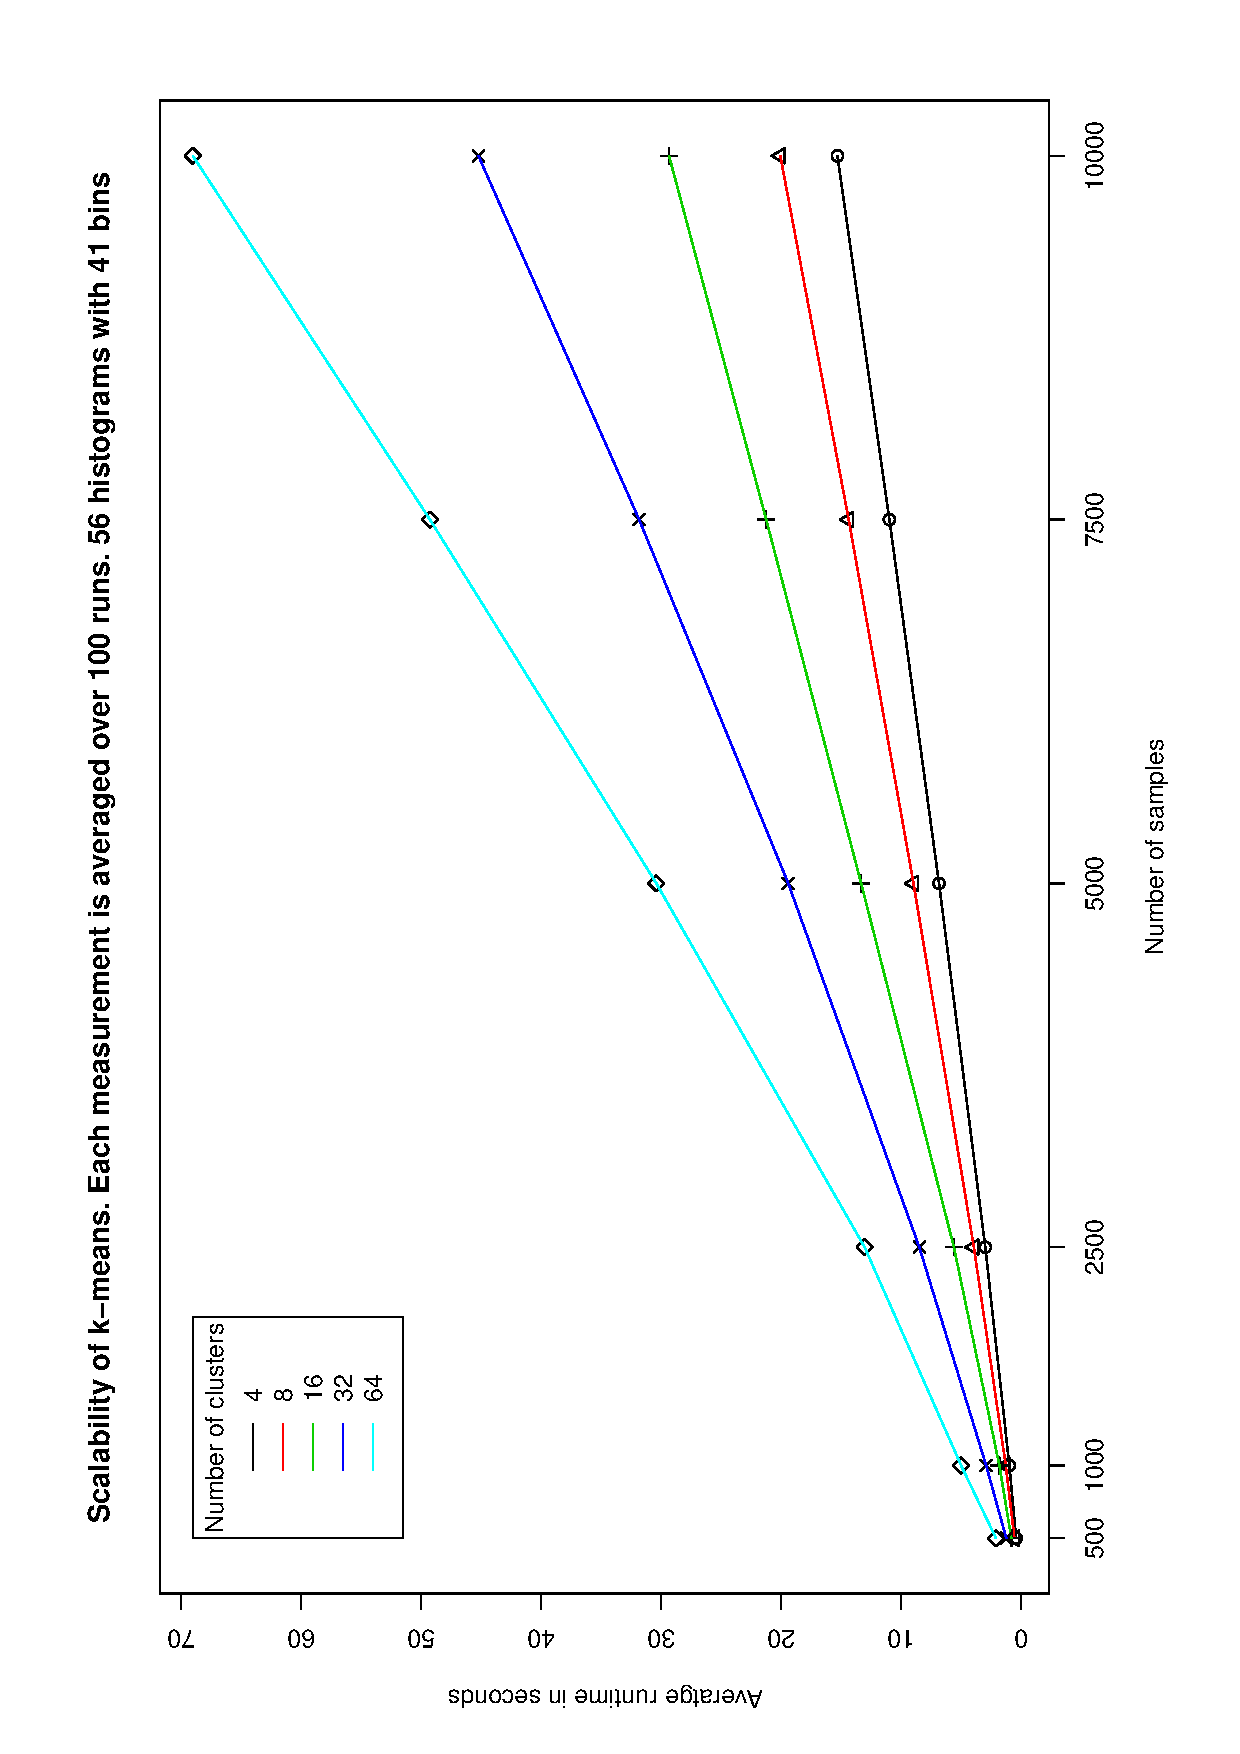
\includegraphics[width=385pt]{Scalability-1_Runtime.pdf}
  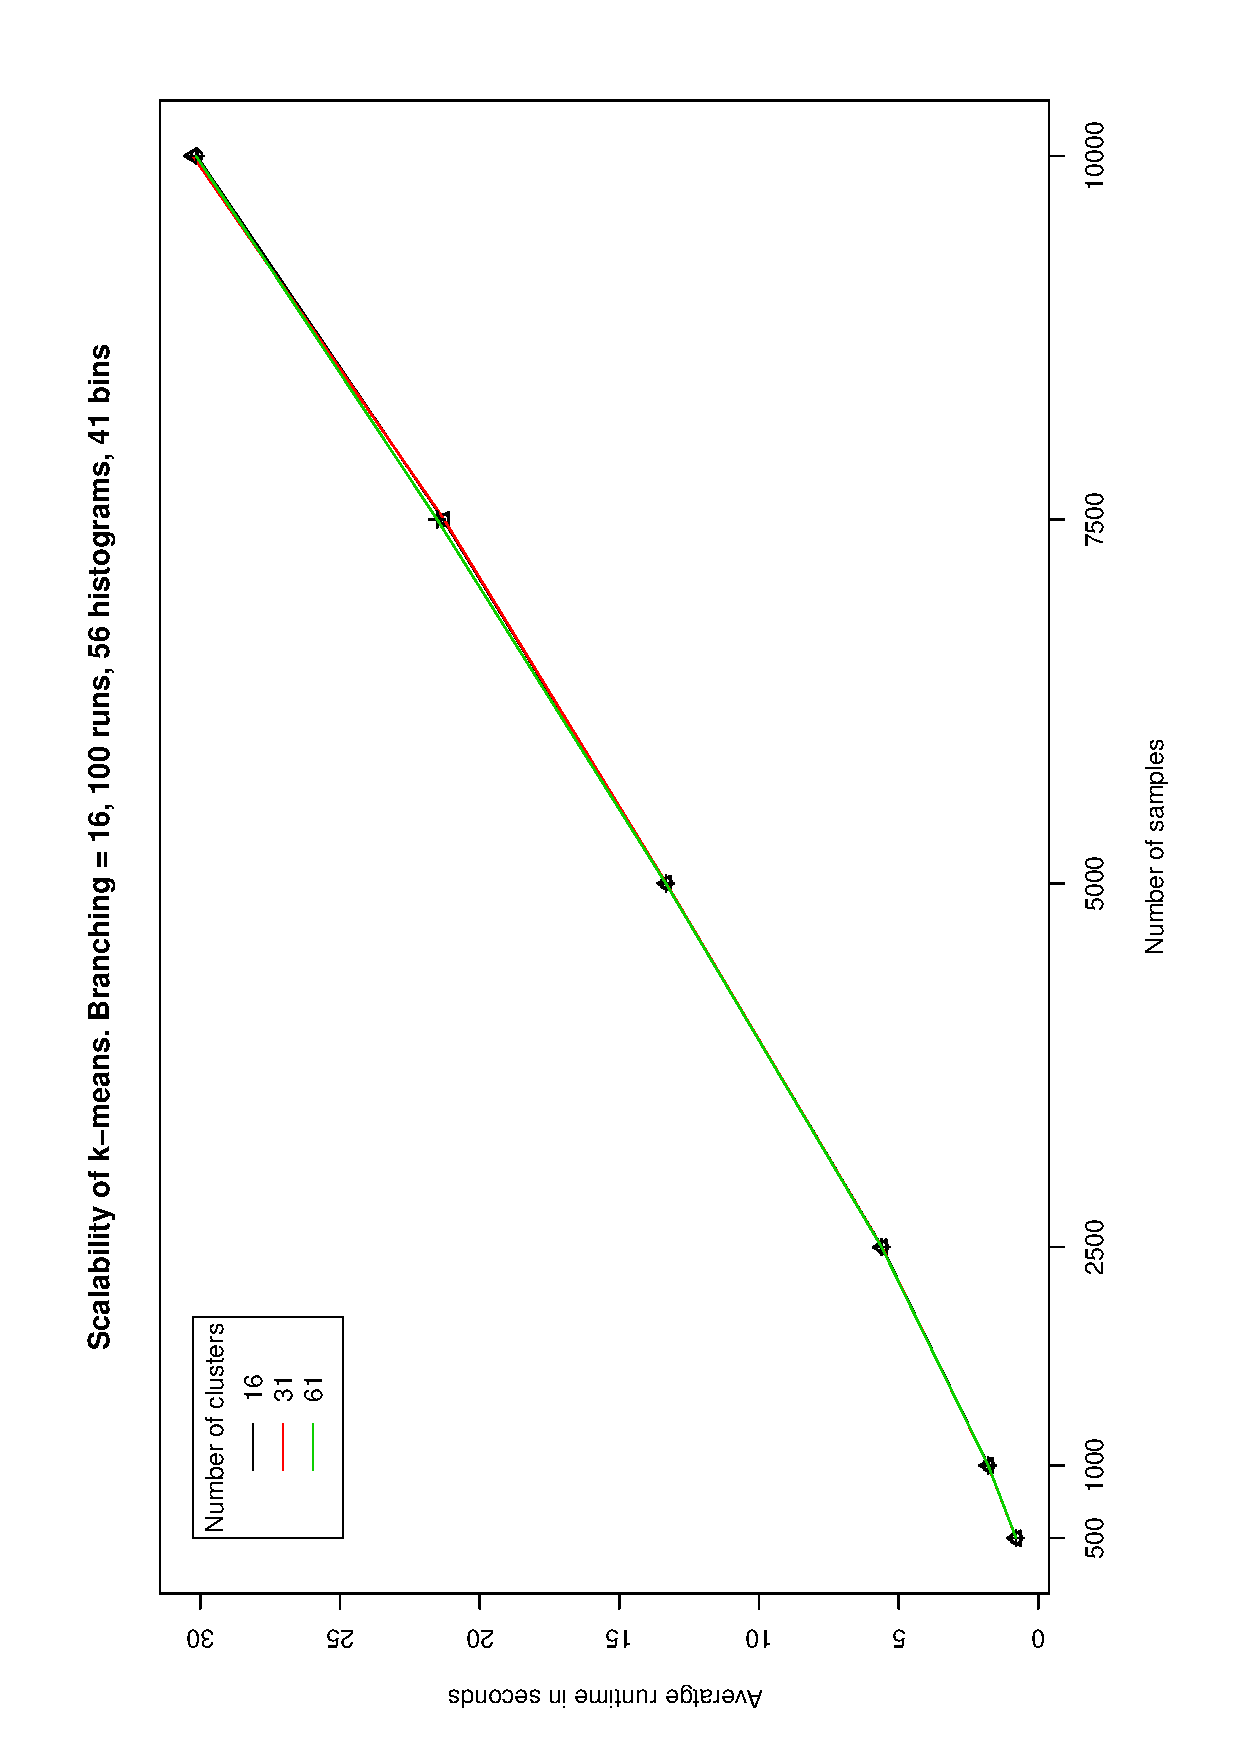
\includegraphics[width=385pt]{Scalability-2_Runtime.pdf}
  \caption{Top: Scalability-1. Bottom: Scalability-2}
  \label{fig:scalability}
\end{figure}

\pagebreak
\section{Profile}
TODO: Display in a way that makes sense.

\end{document}